\documentclass[]{article}
\usepackage{graphicx}
\usepackage{subfig}
%opening
\title{Gu\'ia de creaci\'on de Kernel - TP ARQUI - ITBA}
\author{Lpinilla}
\date{30 Octubre 2018}

\begin{document}

\maketitle

\begin{abstract}
	Este documento es una guía para ayudar en el desarrollo del\
	kernel en el Trabajo Práctico de la materia Arquitectura de\
	las computadoras. 
	\underline{\textit{Disclaimer:}} Este documento no fue revisado por ning\'un miembro de la c\'atedra. Puede contener errores. Queda en su propia responsabilidad utilizar el contenido de este documento.
\end{abstract}

\subsection*{Consideraciones previas}w to enable
Las versiones de Ubuntu mayores a 16.04 presentan problemas al querer manipular la IDT, se recomienda utilizar Docker \textbf{\underline{desde cero.}}

\section*{PIC (Programmable Interface Controller)}
Lo primero que hay que entender es que las computadoras tienen 2\
PIC. El "MasterPIC" y el "SlavePIC". el slave esta "colgado" del\
master (cascading), por lo tanto se puede deshabilitar o ignorar\
lo que venga de él desde el master (IRQ02).\\
Cada PIC tiene 2 entradas, una para leer los datos y otra para conf
igurarlos, el master esta en 0x21 y 0x20. El slave en 0xA1h y 0xA0
respectivamente.

\section*{IRQ}
Cada PIC tiene 8 entradas, 1 bit por cada entrada $\longrightarrow$ 2bytes para configurarlo.

Las entradas del IRQ son:
\begin{center}
	\begin{tabular}{ |c|c| }
		\hline
		IRQ & Descripción\\
		\hline
		\multicolumn{2}{|c|}{MasterPIC} \\	
		\hline	
		0 & Timer-Tick\\
		1 & Keyboard \\
		2 & Cascade (used internally by the two PICs. never raised) \\
		3 & COM2 (if enabled)  \\
		4 & COM1 (if enabled)  \\
		5 & LPT2 (if enabled)  \\
		6 & Floppy Disk  \\
		7 & LPT1 / Unreliable "spurious" interrupt (usually)  \\
		\hline
		\multicolumn{2}{|c|}{SlavePIC} \\	
		\hline	
		8 & RTC \\
		9 & Free for peripherals / legacy SCSI / NIC  \\
		10 & Free for peripherals / SCSI / NIC  \\
		11 & Free for peripherals / SCSI / NIC  \\
		12 & PS2-Mouse \\
		13 & FPU / Coprocessor / Inter-processor  \\
		14 & Primary ATA Hard Disk  \\
		15 & Secondary ATA Hard Disk  \\
		\hline
	\end{tabular}
\end{center}

\section*{Masking del PIC}
Para cambiar la configuración del PIC tenemos que hacer un masking de bits.
Para deshabilitar algo, tenemos que ponerlo en 1, en caso contrario esta habilitado.

Supongamos que queremos solamente habilitar el teclado, para eso habría que
solamente dejar en 0 el bit 1 del MasterPic. Para eso debemos encontrar el valor
en hexa que deja al primer byte del pic en 1101.

Recordando que cada PIC tiene 2 bytes para configurarlo, tenemos que hallar el valor.

En este caso, queremos que este todo en 1 menos el anteúltimo bit: 1111-1101.
La primer parte corresponde al valor F mientras que la segunda al D. Por lo tanto,
el valor a mandarle al MasterPIC es FD.

\begin{verbatim}
	picMasterMask:
	push rbp
	mov rbp, rsp
	mov ax, di
	out	21h,al
	pop rbp
	retn
\end{verbatim}

Análogamente configuramos el slavePIC con el valor FF para no habilitar ninguna
otra interrupcion.

\section*{Interrupciones de Hardware}

Recordando que una interrupci\'on es un evento externo que ocurre, veamos como podemos
realizar driver de un periférico específico (el teclado).

\subsection*{Cadena de ejecuci\'on de interrupciones}
Veamos como resuelve la pc cuando se interact\'ua con el teclado.

\begin{center}
	\begin{enumerate}
		\item Se aprieta una tecla en el teclado.
		\item El teclado activa una interrupci\'on al PIC.
		\item El PIC recibe la interrupci\'on desde el IRQ01 y se
		fija si la deja pasar o no.
		\item Si la deja pasar, le indica al procesador que tiene una interrupci\'on.
		\item El procesador le indica si esta listo o no para recibir interrupciones.
		\item Si esta listo, le env\'ia, el PIC le env\'ia cual de sus interrupciones se activ\'o.
		\item El microprocesador con esa informaci\'on va a buscar a la IDT el registro correspondiente a la interrupci\'on IRQ01.
	\end{enumerate}
\end{center}

En la IDT, el PIC est\'a mapeado directamente, osea que IRQ0 arranca en X0h, IRQ1 en X1h, ... donde X en principio es 0\
Pero acá hay un problema ya que las primeras 32 entradas de la IDT son excepciones
por lo tanto se pisar\'ian las entradas, por eso, se "mueve" el inicio de las IRQ.
En este caso ser\'ia simplemente que X valga 2.\\

Por lo tanto, la tabla de los IRQ arranca en 20 (32 en hexa).

\subsection*{Creaci\'on de Interrupciones}
Para crear un driver tenemos que manejar las interrupciones del perif\'erico (ej Teclado).
Para eso, tenemos que hacer un par de cosas:

\begin{center}
	\begin{enumerate}
		\item Crear la entrada en la IDT.
		\item En la entrada de la IDT, asignar un puntero a funci\'on que va a ser la rutina
		de ejecuci\'on de la interrupci\'on.
		\item De ser necesario, llamar desde la rutina a una funci\'on en C.
	\end{enumerate}
\end{center}

Por ejemplo: Se crea la interrupci\'on en la entrada 21h. $\longrightarrow$ la interrupci\'on llama a la rutina de asm $\longrightarrow$ la rutina llama a una funci\'on de C que se encarga de interactuar con la lectura del teclado.\\

Hay que entender que la rutina apuntada por la IDT no es lo que finalmente ser\'a lo que lee del teclado, esta rutina llama a una funci\'on de C que se va a encargar de eso y de proveer m\'as funcionalidades.

\section*{Excepciones}

Las excepciones son interrupciones que lanza el mismo procesador, por eso, se crean de la misma manera que las interrupciones.

Esta es una tabla con las excepciones m\'as comunes.

\begin{center}
	\begin{tabular}{ |c|c| }
		\hline
		C\'odigo & Decripci\'on\\
		\hline
		0h & Division By zero\\
		1h & Single-step interrupt (see trap flag) \\
		2h & NMI\\
		3h & Breakpoint (callable by the special 1-byte instruction 0xCC, used by debuggers) \\
		4h & Overflow\\
		5h & Bounds\\
		6h & Invalid Opcode \\
		7h & Coprocessor not available \\
		8h & Double Fault\\
		9h & Coprocessor Segment Overrun (386 or earlier only) \\
		Ah & Invalid Task State Segment \\
		Bh & Segment not present \\
		Ch & Stack Fault \\
		Dh & General Protection Fault\\
		Eh & Page Fault\\
		Fh & reserved\\
		10h & Math Fault \\
		11h & Alignment Check \\
		12h & Machine Check \\
		13h & SIMD Floating-Point Exception \\
		14h & Virtualization Exception \\
		15h & Control Protection Exception \\
		\hline
	\end{tabular}
\end{center}

\section*{Teclado}
Una vez que se pueda leer del teclado y mostrar lo que se aprieta, podemos ver que las teclas
no corresponden con lo que se escribe, esto es debido a que falta hacer un mapeo 1:1 con el teclado y sus respectivos valores. \\

Para resolver esto simplemente tenemos que tener el mapa de teclado y mapear las teclas antes de devolverlas.

\section*{Entradas comunes}
Entradas m\'as utilizadas cuando se lee en asm.
\begin{center}
	\begin{tabular}{ |c|c| }
		\hline
		Entradas & Dispositivo\\
		\hline	
		20-21h & MasterPIC\\
		A0-A1h & SlavePIC\\
		60-64h & Keyboard\\
		70-71h & RTC\\
		\hline
	\end{tabular}
\end{center}

\section*{Pasaje de Par\'ametros en 64 bits}
Este es el orden en el que se pasan

\begin{center}
	\begin{enumerate}
		\item rdi.
		\item rsi.
		\item rdx.
		\item rcx.
		\item r8.
		\item r9.
	\end{enumerate}
\end{center}

\section*{Modo de video}

El modo de video es una forma distinta de leer la pantalla por parte del driver del monitor.

El est\'andar VGA-VESA nos permite varios modos de video para elegir, los distintos est\'andares suelen estar compuesto por lo siguiente:

	\begin{enumerate}
		\item Aspect Ratio.
		\item Display Size.
		\item Display Resolution.
		\item Color depth.
		\item Refresh Rate
	\end{enumerate}

Cada est\'andar distinto provee distintas opciones para estos items.\\

Para el TP, como tenemos que hacer un juego, voy a elegir el "Modo 13h" que fue bastante utilizado en videojuegos en su \'epoca por tener un f\'acil acceso a memoria ("Chunky Graphics").\\

Siguiendo una documentaci\'on en internet, para cambiar el modo el modo 13, tengo que poner AH en 00h y en AL el modo que quiero, en este caso AX quedar\'ia: 0x0013h (o sino 4F02 en AX para el SVGA) \\

\textbf{Para entrar en modo video tengo que cambiar el byte $"cfg_vesa"$ a 1 en Pure64/src/sysvar.asm}\\

En el mismo archivo podemos encontrar toda la informaci\'on de VESA bajo el comentario del mismo nombre.

Para cambiar el modo, hay que hard-codear la instrucci\'on en asm dentro de Pure64/src/Pure64.asm simplemente basta con poner:

\begin{verbatim}
;cambiar el modo 13h
mov ax, 0x13
int 0x10

\end{verbatim}

La resoluci\'on de este modo es 320x200px. Es importante recordar el n\'umero 320 (o 3200) ya que lo vamos a ver varias veces.\\

\textit{Una idea para testear:} El cambio de modo lo hacemos con la interrupci\'on 10h del BIOS que despu\'es nuestra IDT pisa.. se podr\'a cambiar de lugar esa interrupci\'on? Si efectivamente se puede cambiar de lugar el puntero de la rutina de ejecuci\'on de la entrada 10, podr\'ia cambiar de modo texto a modo video cuando quiera usando mi propia interrupci\'on.

La pantalla generalmente puede ser descripta por los siguientes valores:\\

\begin{tabular}{ |c|c|}
	\hline
	Width & Cuantos pixels hay en una linea horizontal\\
	Height & Cuantas lineas horizontales hay\\
	Pitch & Cuantos bytes en VRAM hay que saltear para ir un pixel abajo\\
	Depth & Cuantos pixeles de colores se tiene\\
	PixelWidth &  Cuantos bytes en VRAM hay que saltear para ir un pixel a la derecha\\
	\hline
\end{tabular}

\subsection*{Conocimiento General}

Escribir al monitor es s\'implemente escribir de una forma espec\'ifica a una direcci\'on de memoria. En este caso la direcci\'on de memoria es 0xB8000 (sacada del manual de Pure64).\\

La forma en la que tenemos que escribir es B,R,G con las letras que corresponden a Blue, Red y Green. Si te preguntas por qu\'e ese formato y no el m\'as conocido (rgb) es por el \'orden en que se compone el n\'umero. El color originalmente es un n\'umero que tiene todo junto sus valores de rgb, por ejemplo el n\'umero puede que tenga esta forma 0x255255255. En este caso estar\'amos metiendo el color (255,255,255) que representa al 1.\\

La forma en la que compacta el n\'umero es por medio de shifteos. Hace color \& 255 para obtener el azul, (color $<<$ 8) \& 255 para obtener el verde y (color $<<$ 16) \& 255 para obtener el rojo. Esto no es propio del mode 13h sino que todos los modos hacen esto

\subsection*{Imprimir mis propios caracteres}
Para imprimir mis propios tengo que tener el dibujo de cada caracter, ese dibujo se suele hacer en formato de bitmap. Esto funciona de la siguiente manera: \\

la matriz de datos:\\
\begin{center}
1111\\
1000\\
1111\\
\end{center}

podría representar la forma del caracter "C". Entonces lo que tenemos que hacer es tener para cada caracter su mapa (bitmap) y hacer algo simple como:

\begin{verbatim}
for(int i = 0; i < altura_char; i++){
for(int j = 0; j < ancho_char; j++){
if( hay un 1){
pintar_con_un_color(x,y,color);
}
}
}
\end{verbatim}


Obviamente podemos ver que esto no es muy eficiente.\\

\subsection*{Bitmap Encoding}
Como se pudieron dar cuenta, lo anterior si bien funciona, puede ocupar mucho espacio en memoria. Entonces lo que podemos hacer es armar un tipo de codificaci\'on sencillo para codificar las filas del bitmap (este es uno de varios m\'etodos para codificar).\\

Sabiendo que en realidad un char (est\'andar) ocupa 8 bits de largo y 16 bits de algo, eso significa que tenemos 16 filas de 8 bits (o 1 byte). Entonces si podemos codificar cada fila ya ser\'ia mejor.\\

Siguiendo con el ejemplo anterior de la "C" (en este caso nuestro char ser\'ia de 4x3). Podr\'iamos codificar cada fila por el valor num\'erico que representan esos bits, en este caso ser\'ia:\\
0xF\\
0x8\\
0xF\\
Entonces de esta manera tenemos codificado el bitmap.

\subsection*{Optimizaci\'on}
Verificar de a 1 bit a la vez e imprimir 1 pixel es algo sumamente ineficiente, m\'as sabiendo que cada char ocupa 1 byte de largo, entonces nos podemos preguntar: Por que no ir copiando directamente de a bytes?\\

Esto se puede hacer pero es mucho m\'as dif\'icil ya que se tendr\'ia que "empaquetar" (shifteando bits) el color deseado para que se imprima en todos los bits correspondientes


\section*{Programaci\'on de videojuegos en bajo nivel}
En nuestra consigna de TP nos toc\'o realizar el juego PONG pero las t\'ecnicas que vamos a explicar sirven otros tipos de juegos tambi\'en.\\

Antes (80's 90's) los juegos se hac\'ian en Assembler porque las computadoras (y despu\'es las consolas) no pod\'ian procesar algo de alto nivel como C o no era conveniente (solo hab\'ia 40kb de RAM) , a medida que mejoraron las tecnolog\'ias, les permitieron a los desarrolladores poder programar en Assembler pero cuando deb\'ian realizar alguna configurac\'ion como por ejemplo cambiar el color de texto, ten\'ian que cambiar par\'ametros mediante llamadas a ASM.\\

Con el TP tenemos un caso parecido, podemos programar toda la l\'ogica en C pero para poder graficar tenemos que hacerlo mediante syscalls (o creando una librer\'ia que se maneja con las syscalls) para no toca la memoria directamente.\\

Las distintas "partes" de un juego de este estilo son
\begin{enumerate}
	\item Ciclos del juego.
	\item L\'ogica del juego.
	\item Parte gr\'afica del juego.
\end{enumerate}

El o los ciclos del juego es el ciclo principal que va a estar corriendo mientras se est\'e ejecutando el programa. Adentro de este ciclo puede existir una m\'aquina de estados para guiar al jugador mientras se ejecute ("men\'u", "en juego", "fin del juego").\\

La l\'ogica del juego es donde va a estar toda la programaci\'on de la jugabilidad, en nuestro caso, el puntaje, el control de las teclas para jugar y la "f\'isica" de la pelotita que rebota.\\

La parte gr\'afica es la que se encarga de dibujar todo. En bajo nivel, dependiendo el juego, esto podr\'ia a llegar a ser m'as complicado que la l\'ogica del juego ya que tenemos que recordar que no tenemos forma de "pintar" cosas m\'as que llamando a las syscalls y recordando que si cambiamos lo que el usuario esta viendo mientras lo esta viendo, puede generar errores conocidos como "tearing" o "flickering".

\subsection*{Double Buffering o Page Flipping}

\begin{figure}
	\centering
	\subfloat[Double Buffering]{\label{ref_label1}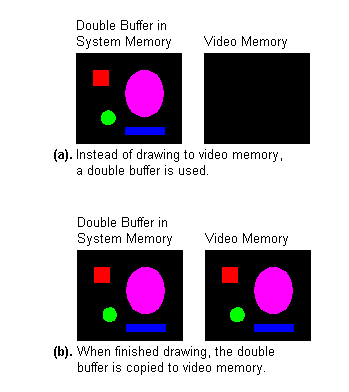
\includegraphics[width=0.5\textwidth]{screenshot001}}
	\subfloat[Page Flipping]{\label{ref_label2}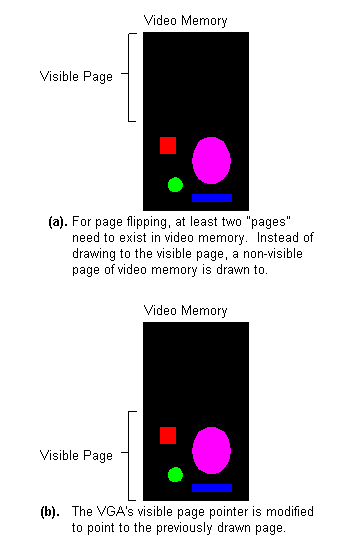
\includegraphics[width=0.4\textwidth]{screenshot002}}
	\caption{\label{ref_label_overall}Overall caption}
\end{figure}


El Double Buffering y el Page Flipping son dos t\'ecnicas conocidas que se encargan de hacer lo mismo de manera distinta. La idea es que en vez de modificar la pantalla mientras se esta mostrando, se utilice una zona de memoria auxiliar para que ser\'ia nuestra "segunda" pantalla.\\

En Page Flipping, si la memoria es lo suficientemente grande, podr\'iamos llegar a tener parte de la memoria que el monitor no esta "viendo", entonces cuando este se llena o queremos cambiarlo, podemos decirle que "mire" a la otra parte que cambiamos.\\

Nosotros vamos a implementar Double Buffering porque VGA Mode 13h no tiene espacio suficiente asignado para "m'as de una pantalla", as\'i que lo primero que hacemos es declarar un array de char[] del tamaño de la resoluci\'on (en nuestro caso, 320 * 200) que va a actuar como nuestro segundo buffer o "shadow\_buffer".\\

Dependiendo de las especificaciones, podemos hacer las cosas m\'as o menos eficiente. Mode 13h no nos deja simplemente cambiar el puntero a su direcci\'on de memoria as\'i que tenemos uqe copiar todo el buffer cuando queremos "cambiarlos". Con Page Flipping habr\'ia que ver si el modo nos deja cambiar el puntero o hay que tambi\'en copiar de una zona de memoria a otra.



\end{document}